%% ----------------------------------------------------------------------------
% BIWI SA/MA thesis template
%
% Created 09/29/2006 by Andreas Ess
% Extended 13/02/2009 by Jan Lesniak - jlesniak@vision.ee.ethz.ch
%% ----------------------------------------------------------------------------
\documentclass[pdftex,11pt,openright,headsepline]{book}

\usepackage{paralist}		% List environment
\usepackage{color}		% For colored text
\usepackage{times}
\usepackage{amsfonts}		% Additional math fonts
\usepackage{amsmath}		% Math symbols
\usepackage{latexsym}
\usepackage{graphicx}		% For including images
% \usepackage{subcaption}
% \usepackage{listings}		% If listings are needed
\usepackage{mydefs}		% Some of our own definitions
% \usepackage{wrapfig}		% To wrap images
% \usepackage{algorithmic}	% Nice algorithm environment
% \usepackage{algorithm}
\usepackage{fancyhdr}		% Produce the nice header
\usepackage{fullpage} % Use the full page
\usepackage{tikz} % For plots
\usepackage{pgfplots} % For plots
\usepackage{pgfplotstable} % For plots
\pgfplotsset{compat=newest} % For plots
\usetikzlibrary{plotmarks} % For plots
\usepgfplotslibrary{colorbrewer} % Nice colors
\pgfplotsset{cycle list/Set2-8}


% Change the appearance of the header. Here \MakeUppercase is hard-coded, so renewing this command allows to elegantly change the header appearance.
\renewcommand{\MakeUppercase}{\scshape}

% Set the headings' appearance in the ``fancy'' pagestyle
\fancyhead{}
\fancyhead[RO, LE]{\leftmark}
\fancyfoot{}
\fancyfoot[RO, LE]{\thepage}

% The first pages shall be empty, even no page numbering


\begin{document}
\pagestyle{empty} % even no page number

\fancypagestyle{plain}{
  \renewcommand{\headrulewidth}{0.0pt}
  \fancyfoot{}
  \fancyhead{}
}

% Title page, modify accordingly
%!TEX root = ../thesis.tex

\begin{titlingpage}
\begin{center}

\begin{figure}
  
\includegraphics[trim={0 6cm 0 4cm},clip,width=1\linewidth]{figures/cvl_logo.pdf}
\end{figure}

{\fontencoding{OT1}\fontfamily{pplx}\selectfont
\large{\textsc{Eidgen\"ossische Technische Hochschule Z\"urich\\[1mm]
Computer Vision Laboratory\\[25mm]}}

\huge{\textsc{Video Object Segmentation by \\ Tracking One Point}}
\vskip 0.5cm
\hrule
\vskip 2.6cm

\Large
by \textsc{Alberto Montes G\'omez}\\[2cm]

\large
Advisors: Dr. Jordi Pont-Tuset, Kevis Maninis, Sergi Caelles\\
Director: Prof. Luc Van Gool\\
Z\"urich, April 2018}
\end{center}
\end{titlingpage}

\cleardoublepage

%!TEX root = ../thesis.tex

%% ----------------------------------------------------------------------------
% BIWI SA/MA thesis template
%
% Created 09/29/2006 by Andreas Ess
% Extended 13/02/2009 by Jan Lesniak - jlesniak@vision.ee.ethz.ch
%% ----------------------------------------------------------------------------


\chapter*{Abstract}
\label{cha:abstract}

\noindent The abstract gives a concise overview of the work you have done. The reader shall be able to decide whether the work which has been done is interesting for him by reading the abstract. Provide a brief account on the following questions:

\begin{itemize}
 \item What is the problem you worked on? (Introduction)
 \item How did you tackle the problem? (Materials and Methods)
 \item What were your results and findings? (Results)
 \item Why are your findings significant? (Conclusion)
\end{itemize}

\noindent The abstract should approximately cover half of a page, and does generally not contain citations.


% Input here any acknowledgements
%!TEX root = ../thesis.tex

\chapter*{Acknowledgements}
\label{cha:ack}

In the first place, I would like to thank Dr. Jordi Pont-Tuset for allowing me to do my master thesis with the segmentation group at Computer Vision Lab. 
In extension I would like to thank Kevis Maninis and Sergi Caelles for their advisory work. 
I am very gratefully to them all for their patiente and guidance during this Master Thesis. 
They also have teached me how to do research in the Computer Vision field.

From ETH Z\"urich, I would like to thank Prof. Luc Van Gool for giving me the opportunity to perform research in the Computer Vision Lab.
In addition I would like to thank all the professors I had from the courses taken, from which I have learned a lot.

From UPC Barcelona, I would like to mention Prof. Xavi Gir\'o-i-Nieto, Amaia Salvador and Santiago Pascual from the Image Processing Group. 
Was with them, when I was performing my Bachelor Thesis, that I was introduced to Computer Vision and Image Processing and they supported me to pursuing my studies in this field in ETH Z\"urich.

I would also like to thank my girlfriend Judith Bergad\`a for all his support given to me during the development of my studies and this thesis and pushing me forward.

Finally, I would like to thank my family for their constant support and motivate me during my studies. 

\cleardoublepage
\newpage

% Chapter-pages etc. use the ``plain'' pagestyle - since we don't want to have a heading at all at chapter-pages, redefine plain accordingly. Don't forget the page number.
\fancypagestyle{plain}{
  \renewcommand{\headrulewidth}{0.0pt}
  \fancyfoot{}
  \fancyfoot[RO, LE]{\thepage}
  \fancyhead{}
}

\pagestyle{fancy}
\pagenumbering{Roman}

% Insert table of contents
\tableofcontents

% Insert list of figures
\listoffigures
\cleardoublepage

% Insert list of tables
\listoftables
\cleardoublepage

\newpage

\pagenumbering{arabic}

%% ----------------------------------------------------------------------------
% Actual text comes here - defer it to other files and use \input{bla.tex}, ..
%% ----------------------------------------------------------------------------
%!TEX root = ../thesis.tex

\chapter{Introduction}
\label{cha:introduction}

During the last decade, Computer Vision has grown in popularity as a tool to perform tasks as humans do.
Moreover, with the introduction of deep learning techniques, which try to mimic how the human brain works, the field has experienced an explosion on speed and performance which has fostered a lot of research in the topic.

Furthermore, many companies use these techniques in products related to image and video processing software, video classification at video portals or language translation.

% But the explosion of products using computer vision techniques is just beginning, as for example autonomous driving is just around the corner and rely on this techniques to provide which can be a huge revolution in humanity.
% Thus, this is an exciting field to work nowadays as it will help to solve new problems arising and provide us with great products.
Thus, this is an exciting field to work nowadays as new results can be around the corner and can lead us to new products.


This thesis focuses on the task of video object segmentation.
We refer to segmentation as the partition of pixels from a video in different classes.
These classes will be different instances appearing in the video plus the background.
This is an important task in the Computer Vision field during the lasts years and can be a core block for numerous applications like video editing and post-processing, video retrieval, activity recognition and much more.

In previous works, there have been mainly two different approaches to tackle this problem, unsupervised or semi-supervised.
In the unsupervised methods, the model tries to infer which instances or objects are the protagonists during the whole video and then outputs a segmentation mask for each instance.
On the other hand, in the semi-supervised methods, the instances that we want to segment are given to the model in the form of the mask in the first frame.
Thus, the model already has information about the objects that need to be be segmented and can propagate this initial mask through all the sequence to output a prediction.
% Talk about them

Our proposed method during this thesis tries to solve the problem of video object segmentation from a new perspective.
It is a weakly supervised approach which instead of using the whole mask of the instance to segment, a single point per instance is given.
This approach presents some benefits when applied to real applications, as point annotations are easier and faster to obtain than full mask segmentations.
% Developing a method which tries to solve this problem with this approach may lead to some utility in real applications as points annotations are more easy and fast to perform rather than a full segmentation mask on the first frame.


Our proposed method performs two tasks and fuses them to obtain a final prediction: point tracking and instance segmentation from a point.
With point tracking, we are able to keep track at every frame of a point per each instance.
In addition to this, a model has been trained to learn an embedding representation that can be used, given a point and its label, to label the rest of the pixels with a similarity computation.
A combination of these two tasks gives us a method that is capable of performing the task of weakly semi-supervised video instance segmentation.

In order to train and evaluate our method, a dataset is required.
To evaluate our method, we have used the DAVIS~\davisboth{} dataset which provides instance segmentation masks for multiple video sequences.
This dataset is well known in the research community for being a benchmark to evaluate video segmentation models.

In \figref{intro:davis} we can see a sequence and its mask annotation overlaid to it for each instance in the video.

\begin{figure}[h]
  \centering
  \davissequencerow{dogs-jump}{1}{5}{10}{15}
  \davissequencerow{dogs-jump}{20}{25}{30}{35}
  \davissequencerow{dogs-jump}{40}{45}{50}{55}
  \caption{\textit{Dogs Jump} annotated video sequence with all the instance masks overlaid in different colors. }
  \label{fig:intro:davis}
\end{figure}

In addition, the PASCAL~\pascal{} has been used.
It provides segmentation masks for different object instances in images.
This dataset has helped us to train the embedding model to be able to obtain a good pixel representation that knows the difference between two instances of the same class.

This thesis is structured in the following way. First, in \charef{stateofart}, the current state-of-the-art techniques in image and video instance segmentation are reviewed in order to have an idea of the advantages and drawbacks of the other methods.

Then, in \charef{methods}, our proposed method is defined and explained in detail.
After that, in \charef{experimentsandresults}, the different experiments to test our method are detailed in addition to its results.
Finally, in \charef{conclusionsfuturework}, the conclusions about the benefits and drawbacks of our proposed method are explained.

%!TEX root = ../thesis.tex

\chapter{State of the Art}
\label{cha:stateofart}

In this chapter, we summarize the most relevant work on instance object segmentation.
First, we focus on tracking implementations and later we talk about state of the art methods for object instance segmentation and some implementations applied to video.

\section{Tracking}
\label{sec:soa_tracking}

Tracking implementations are mainly focus on video object tracking.
This conists on taking the bounding box sorrounding and object and make bounding box predictions throught the video that contains the object to track.

One state of the art implementation is MDNet~\cite{nam2016learning}.
It proposes a Convolutional Neural Network with shared layers and multiple branches of domain-specific layers.
The architecture overview is showed at Figure~\ref{fig:mdnet}.
Each branch is responsible for binary classification to identify the target in each specific video.
This domain-specific layers are updated online and the online tracking is performed by evaluating the candidate windows randomly sampled around the previous target state.
This showed state-of-the art results on tracking benchmarks and was the winner of the VOT Challenge~\cite{VOT_TPAMI} in 2016.

\begin{figure}[h]
\centering
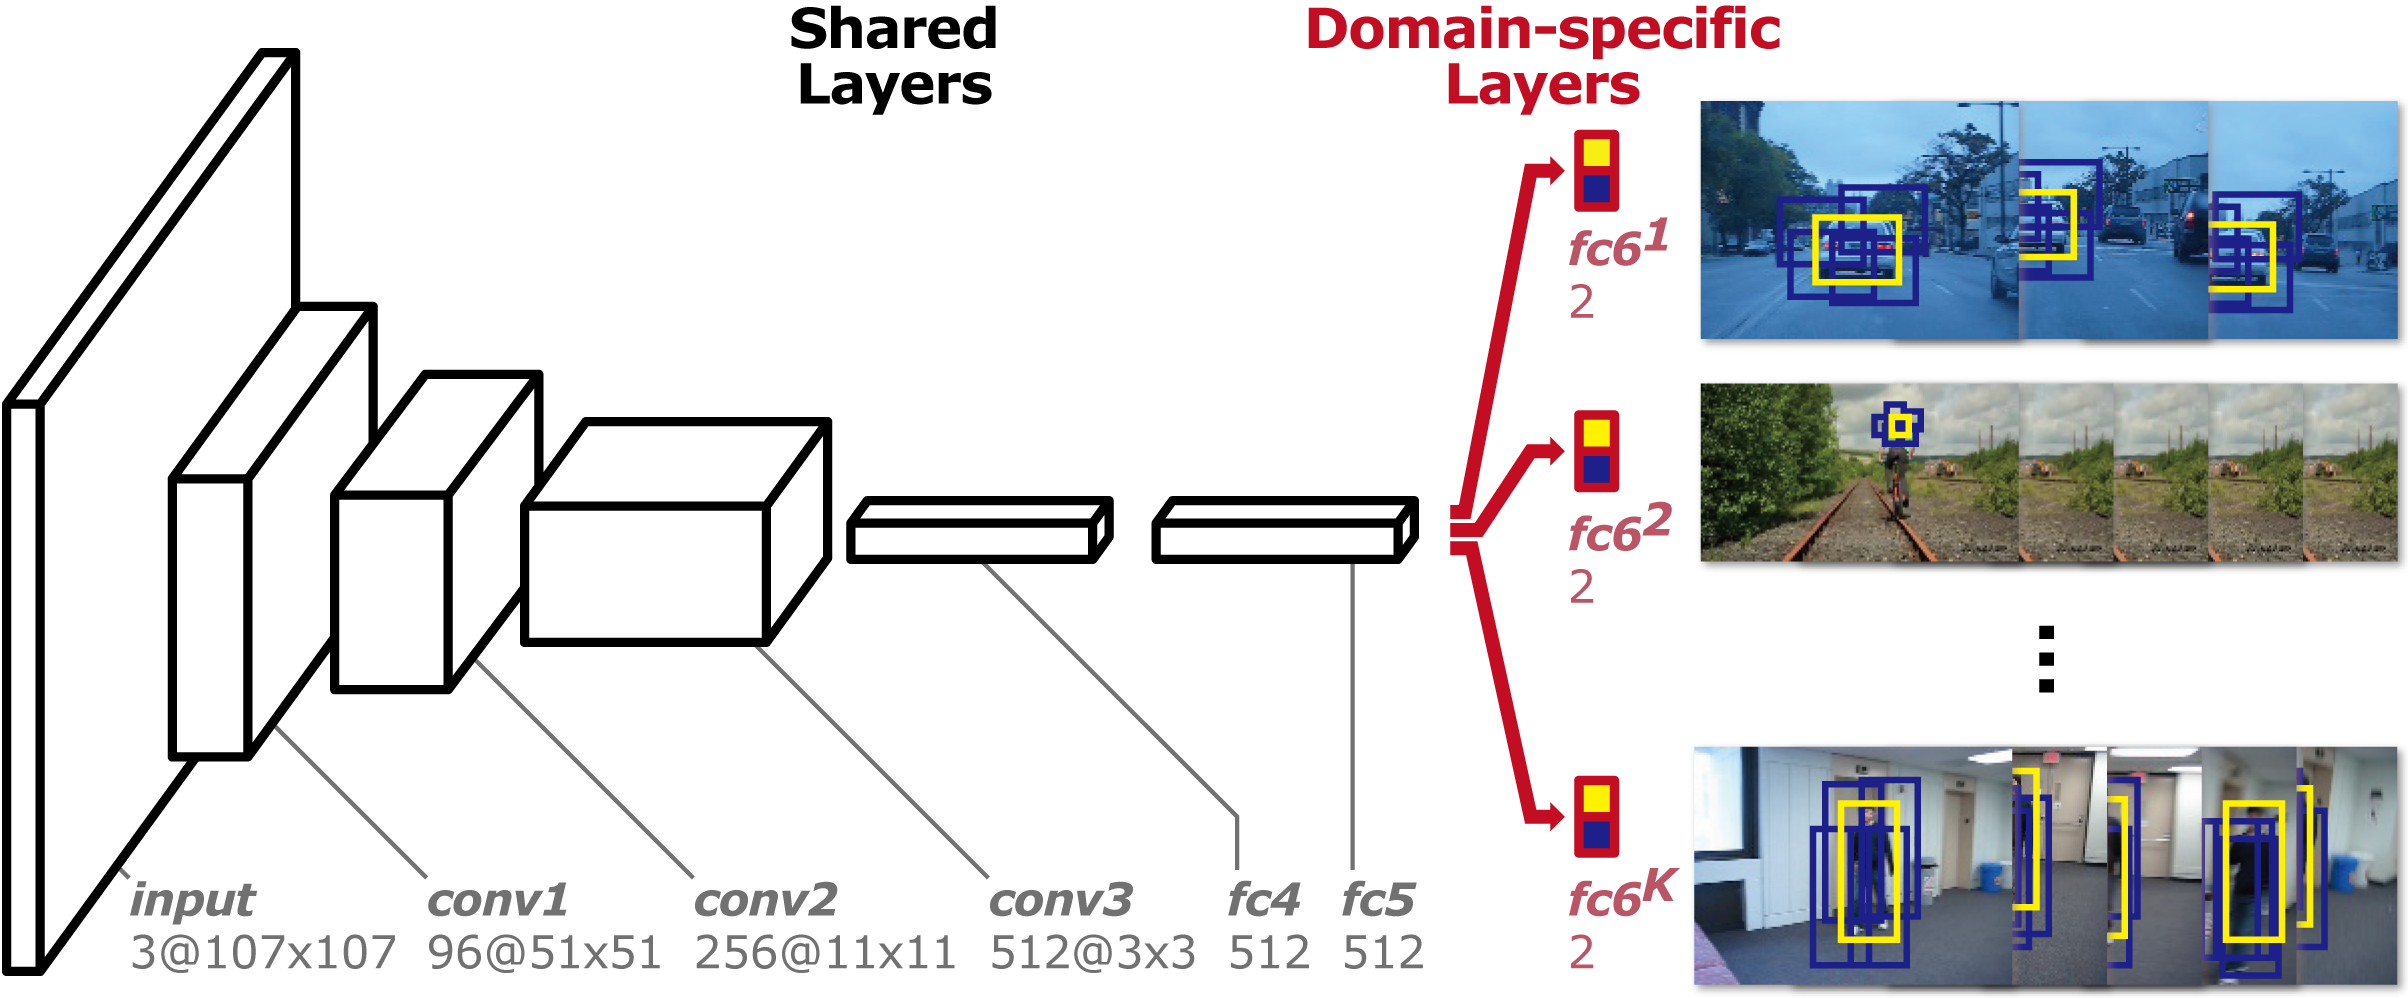
\includegraphics[width=.8\linewidth]{figures/mdnet/architecture.png}
\label{fig:mdnet}
\caption{MDNet architecture. }
\end{figure}

Unfortunetly there are not implementations that focus on keypoints tracking which is the idea behind this thesis.

% Stacked Hourglass Networks for Human Pose Estimation~\cite{newell2016stacked}


\section{Instance Segmentation}
\label{sec:soa_instancesegmentation}

Instance detection and segmentation is one of the most challenging tasks in Computer Vision right now.
In this section we explore some of the works that tackle instance segmentation in different domains like image and video.

\paragraph{Mask R-CNN~\cite{he2017mask}}
This work come from a series of work that started with object detection on images using Convolutional Neural Networks.
With the time they iterate through the architecture to make it differentiable and be able to train it end-to-end, and the last step consisted on predict not only the bounding box of the detected object but its mask.
The idea behind this method consists on a CNN that with a forward pass extract the features at the last convolutional layer.
Then a set of bounding box proposals are generated and the features in each proposed bounding box are used in one branch to predict a objectiveness score and bounding box regressions.
With this branch a set of bounding box are obtained and score predicted. With this values, a second branch is responsible to predict a mask from each proposal.
The final prediction use maximum supression to reduce the proposal to the final prediction masks.
This approach show state of the art results on multiple datasets at the cost of using a very large amount (in the order of 1000) proposals per a single image.

\paragraph{Deep Metric Learning~\cite{fathi2017semantic}}
This works focus also into instance object segmentation on images.
They use a Convolutional Neural Network to predict an embedding representation per each pixel.
This network is trained using metric learning, regressing how likely two pixels are to belong to the same object.
Then they propose the use of seed points to predict the instances and its masks on an image once the embedding for each pixels is computed.

\paragraph{OSVOS~\cite{caelles2017one} and OnAVOS~\cite{voigtlaender17BMVC}}
This works focus on instance segmentation on video.
Their main approach consists on train a parent network that given a frame is able to predict the mask of the foreground (all object instances in the image) and then finetune a network for each video.
This finetune is performed given the mask of the first frame (this methods tackle semi-supervised video object segmentation) and then the trained network for each video is used to predict the masks for the rest of the frames.
The OnAVOS~\cite{voigtlaender17BMVC} work in this last step add an online training. Make predictions of the frames and after each frame predicted the network is online trained with the new predicted mask.
This two implementations present the state of the art results on the DAVIS dataset.

\paragraph{MaskRNN~\cite{NIPS2017_6636}}
This work proposes a recurrent neural network approach which fuses in each frame of the video the output of two deep nets for each objects instance.
The first net is a binary segmentation network providing a mask and the second one is a localization network providing a bounding box.
Thanks to the recurrent component and the localization component, this method is able to take advantage of long-term temporal structures of the video as well as rejecting outliers.
This method also provide competitive results with the previous works of OSVOS~\cite{caelles2017one} and OnAVOS~\cite{voigtlaender17BMVC}.

% \paragraph{Proposal Free Network}~\cite{liang2015proposal}

%!TEX root = ../thesis.tex

\chapter{Methods}
\label{cha:methods}

In this chapter we are going to explain the different methods developed during this thesis.
First, we are going to explain the backbone architecture used during the entire thesis.
Then, we are going to explain how we train a CNN model to track points.
The last section will explain how metric learning works and how we have used it.

\section{Backbone Architecture}
\label{sec:methods:backbonearchitecture}

The objective of this thesis has been to obtain a deep learning model which is capable of, given a point per instance, being able to predict its segmentation through all the videos.
As it is usual on the literature, current best performing deep learning models for computer vision tasks (and more precisely in segmentation) use fully convolutional neural networks.
These models perform convolution operations over the input which is usually an image.

During the development of this thesis, we have used as a backbone architecture the DeepLab~\deeplab{} model for semantic segmentation.
This model is fully convolutional and it is based on the ResNet~\resnet{} architecture which was used for image classification.
The DeepLab model applies a sequence of convolutional layers to the input image, and instead of a classifier, plugs an Atrous Spatial Pyramid Pooling (also defined in~\deeplab{}) at the very last part of the architecture to obtain a segmentation mask.
%what does is to keep the convolutional layers from ResNet~\resnet and add at the end some deconvolutional operations to obtain as an output a mask instead of an object classifier.
Doing this allows the model to be fully convolutional and free of the constraint about the input image size.

The ResNet architecture is based on layers with residual connections.
\figref{backbonearchitecture:resnetblock} illustrates how each bottleneck layer block is built.
Each layer applies some convolutional operations to the input and then adds this result to the original input as a residual.

\begin{figure}[h]
  \centering
  \adjincludegraphics[trim={{.5\width} 0 0 0}, clip, width=.5\textwidth]{figures/resnet/block_deeper.pdf}
  \caption{ResNet~\resnet{} residual block architecture. }
  \label{fig:backbonearchitecture:resnetblock}
\end{figure}

For a more detailed description of the whole architecture of the DeepLab convolutional neural network see \tabref{backbonearchitecture:deeplabarch}, where two versions used are described: ResNet50 and ResNet101.
The architecture takes as input images of size $512 \times 512$ and outputs the input size downsampled by $8$ both in height and width.
Also, note that the number of output channels is 2048, so this output can be used directly, or a header can be plugged.
A header can be any group of layers that perform a task. Some examples could be a group of fully connected layers that can perform a classification,
or a group of convolutional layers that reduce the dimensionality.
In the scenario of this thesis, a header made of a single convolutional filter with kernel size 1 have been used in order to test a dimensionality reduction.
% \ToDo{Explain what a header is} can be plugged to reduce the dimensionality (in the case of classification, reduce the dimensionality to the number of classes).
Because of these, this architecture is very versatile and easy to use with images.

\newcommand{\blocka}[2]{\multirow{3}{*}{\(\left[\begin{array}{c}\text{3$\times$3, #1}\\[-.1em] \text{3$\times$3, #1} \end{array}\right]\)$\times$#2}
}
\newcommand{\blockb}[3]{\multirow{3}{*}{\(\left[\begin{array}{c}\text{1$\times$1, #2}\\[-.1em] \text{3$\times$3, #2}\\[-.1em] \text{1$\times$1, #1}\end{array}\right]\)$\times$#3}
}
\begin{table}[h]
  \centering
  \begin{tabular}{c|c|c|c}
    \toprule
    layer name & output size & 50-layer & 101-layer \\
    \midrule
    conv1 & 256$\times$256 & \multicolumn{2}{c}{7$\times$7, 64, stride 2}\\
    \midrule
    \multirow{4}{*}{conv2\_x} & \multirow{4}{*}{128$\times$128} & \multicolumn{2}{c}{3$\times$3 max pool, stride 2} \\\cline{3-4}
      &  &  \blockb{256}{64}{3} & \blockb{256}{64}{3} \\
      &  &  &\\
      &  &  &\\
    \hline
    \multirow{3}{*}{conv3\_x} &  \multirow{3}{*}{64$\times$64}    & \blockb{512}{128}{4}  & \blockb{512}{128}{4}\\
      &  &  &\\
      &  &  & \\
    \hline
    \multirow{3}{*}{conv4\_x} & \multirow{3}{*}{64$\times$64}  & \blockb{1024}{256}{6}  & \blockb{1024}{256}{23} \\
      &  &  &\\
      &  &  & \\
    \hline
    \multirow{3}{*}{conv5\_x} & \multirow{3}{*}{64$\times$64}  &  \blockb{2048}{512}{3}  & \blockb{2048}{512}{3}\\
      &  &  &\\
      &  &  & \\
    \bottomrule
  \end{tabular}
  \caption{Architectures for DeepLab~\deeplab{} using residual blocks.
    Building blocks are shown in brackets (see also \figref{backbonearchitecture:resnetblock}), with the numbers of blocks stacked.
  }
  \label{tab:backbonearchitecture:deeplabarch}
\end{table}

In the original ResNet architecture downsampling with stride 2 was performed at layers \textit{conv3\_1}, \textit{conv4\_1} and \textit{conv5\_1}.
On DeepLab, the downsampling with stride 2 is only performed at \textit{conv3\_1}.
In contrast, in \textit{conv4\_x} and \textit{conv5\_x} all the convolutions are performed with dilation $2$ and $4$, respectively.
The dilated convolution was presented in~\dilatedconv{} and supports expansion of the receptive field without loss of spatial resolution.


\section{Tracking}
\label{sec:methods:tracking}

In order to track points through a video sequence, one possible approach is to regress the point position in an image using a heatmap.
The point representation is inspired by~\hourglass{} which used heatmaps to predict keypoints positions.
In our experiments, we are going to use the DeepLab ResNet architecture described in \secref{methods:backbonearchitecture} plus an additional module, a PSP~\pspnet{} module that will reduce the output to a single channel image.
This output can be trained to predict the point representation as a gaussian heatmap % using a pyramid scene parsing.\ToDo{Reformulate text}
% This will allow us to regress a heatmap representation of a point
using the Mean Squared Error loss function.

The heatmap is built using the coordinate of a point $p = (p_x, p_y)$ and computing a guassian around this point.
In \equref{tracking:heatmap} is shown how to build a heatmap $\mathcal{H}$ which allows some customization with the parameter $\sigma$ which is the spreadness of the sigma.
Note that the values of the heatmap are bounded between $[0, 1]$.
To observe a graphical example, in \figref{tracking:pointrepresentation} there is a point annotated on an image and the resulting heatmap.

\begin{equation}
  \mathcal{H}(x, y) = \exp \left[ -4 \log(2) \frac{ (x - p_x)^2 + (y - p_y)^2 }{ \sigma^2 } \right]
  \label{eq:tracking:heatmap}
\end{equation}

\begin{figure}[h]
  \centering
  \begin{subfigure}{.5\textwidth}
    \centering
    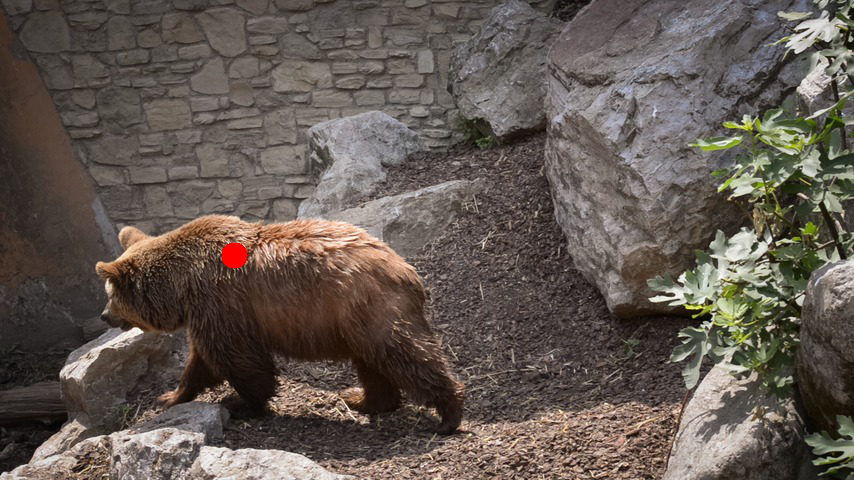
\includegraphics[width=.8\linewidth]{figures/methods/heatmaps/image_point.png}
  \end{subfigure}%
  \begin{subfigure}{.5\textwidth}
    \centering
    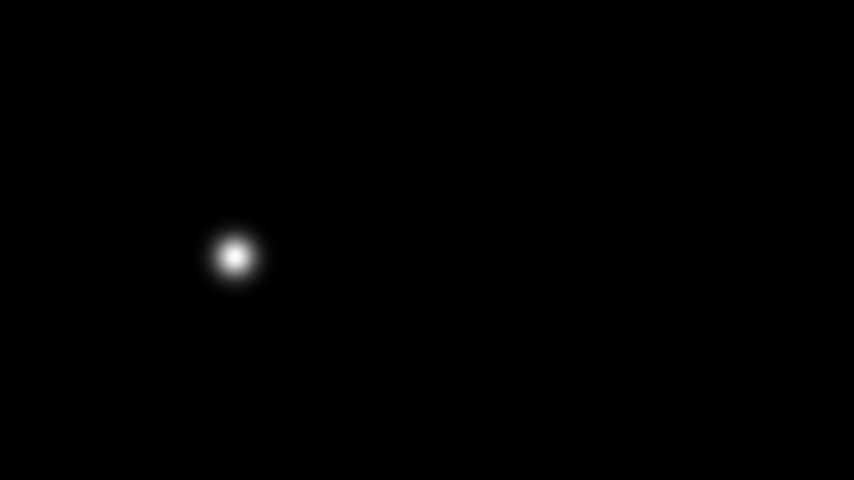
\includegraphics[width=.8\linewidth]{figures/methods/heatmaps/heatmap.png}
  \end{subfigure}
  \caption{
  Point representation.
  \textbf{Left}: Image with the annotated points (image resolution $854 \times 480$ pixels).
  \textbf{Right}: Heatmap to represent the point with $\sigma = 32$ pixels. }
  \label{fig:tracking:pointrepresentation}
\end{figure}

The strategy to train a model that tracks a point given in the first frame will be the same used in OSVOS~\osvos{}.
% TODO: Explain VOC
First is used a model pretrained on semantic segmentation which have learned the representation of all the classes appearing at PASCAL~\pascal{}.
Then this model is finetuned over the first frame of one sequence.
As we only have a single image, some data augmentation is required to enrich the training data and don't overfit on a single image.
Finally we will test each sequence's model with the rest of the frames and extract the predicted tracked point as the coordinate of the heatmap's maximum.
% with Visual Object Classes over the first frame of each sequence.
% Adding some data augmentation to enrich the training, we will test each sequence models with the rest of the frames and extract the maximum of the predicted heatmap as tracked object.

\section{Metric Learning with Triplet Loss}
\label{sec:methods:metriclearning}

Another approach to track a point in a video sequence could consist on training a model which outputs an embedding for each pixel that can be meaningful to obtain instance segmentation.
In order to obtain a good embedding, metric learning has been used.
Metric learning performs the task of learning a good embedding representation using distance comparison.
% distance function over objects, which in our case, the objects are embeddings.\ToDo{Reformulate}

One way to apply metric learning is using a Triplet Loss which was first introduced in~\metriclearning{}.
One famous implementation of this Triplet Loss was used in FaceNet~\facenet{} where they train a model to embed face images and predict similarity between them.

The objective of the Triplet Loss consists on learning a distance difference between triplets of points.
The triplet consists on three points that are called: anchor, positive and negative.
It must fill the condition that the label of the anchor and the positive point are the same, while the label of the negative is different.
The objective of the Triplet Loss is to push the distance of the anchor and positive points to be closer than the distance between the anchor and negative by some margin $\alpha$.
In \figref{tripletloss:visualization} a diagram about the learning procedure is shown.

\begin{figure}[h]
  \centering
  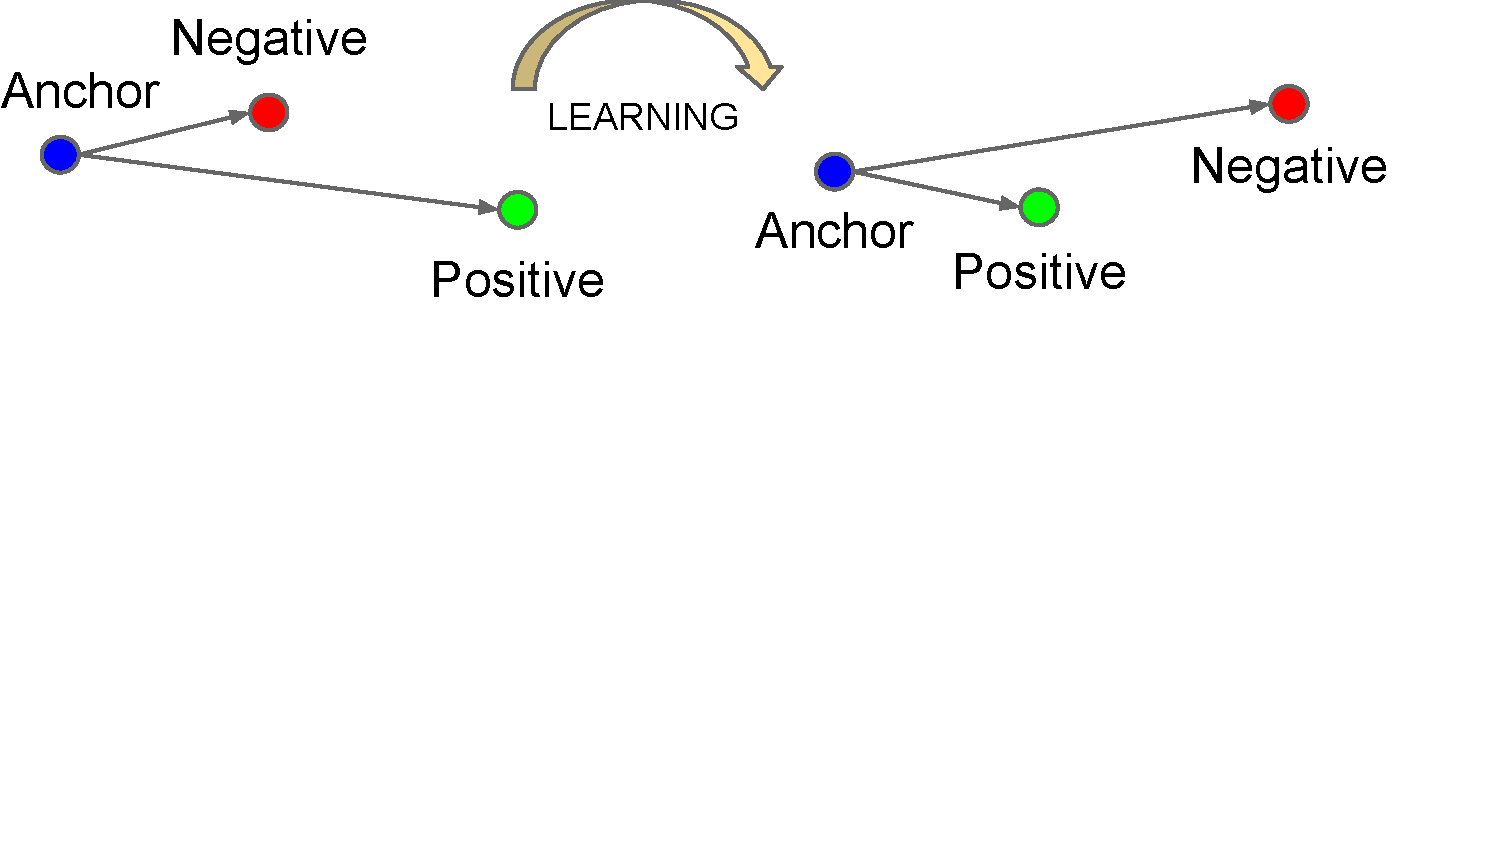
\includegraphics[trim=1cm 10cm 2.5cm 0cm, width=0.7\linewidth]{figures/methods/triplet_loss/triplet_viz.pdf}
  \caption{
    Graphical representation of Triplet Loss learning.
  Figure extracted from~\facenet{}. }
    \label{fig:tripletloss:visualization}
\end{figure}

In our scenario, we use DeepLab~\deeplab{} explained in detail in \secref{methods:backbonearchitecture}.
We use a model that is pretrained for semantic segmentation, and we use the full network except the last classification part which predicts the pixels class.
By default, this model, given an image of size $H \times W$, outputs a feature map of size $H' \times W' = \frac{H}{8} \times \frac{W}{8}$ with $2048$ dimensions.
A convolutional head can be plugged to reduce this dimensionality to a lower dimension $D$ which may lead to a better embedding.

Before giving the equations of the Triple Loss, we define the following notation.
Let $\mathcal{I} \in \mathbb{R}^{H \times W}$ be the input image of size $H \times W$.
The output size of the model will be $H' \times W' = \frac{H}{8} \times \frac{W}{8}$ and the output embedding will be $\mathcal{X} = \{x_i\}^{H' \times W'}$ where $x_i \in \mathbb{R}^D$ is the i-th output pixel embedding.
Let the Convolutional Neural Network be the embedding model $f(\mathcal{I}; \Theta)$ which computes the embedding from a single image:

\begin{equation}
  \mathcal{X} = f(\mathcal{I}; \Theta)
\end{equation}

When training the model,
only the mask of a single object is available,
so the learning only pushes the embeddings of one instance at each time.
% there is available the ground truth mask of one object instance in the image.
When the image is forwarded through the model and the embeddings are computed, $N$ triplets of pixels are sampled.
For each triplet, two pixels belonging to the mask are sampled and assigned as anchor and positive pixels ($x_a$ and $x_p$ respectively).
Finally, a pixel not belonging to the mask is sampled and assigned as negative pixel $x_n$.

\begin{equation}
  \label{eq:tripletloss:1}
  \mathcal{L}_{triplet} = \sum_i^N \max \left( d(x_a^{(i)}, x_p^{(i)}) - d(x_a^{(i)}, x_n^{(i)})  + \alpha, 0 \right)
\end{equation}

The $\alpha$ term on the Triplet Loss is the margin used to enforce the minimum difference between the distance of positive pairs and negative pairs.
$d$ is the distance function, which in our case the $l^2$ norm is used.
So \equref{tripletloss:1} will end up as follows:

\begin{equation}
  \label{eq:tripletloss:2}
  \mathcal{L}_{triplet} =
	\sum_i^N \max \left(
		\|x_a^{(i)} - x_p^{(i)}\|_2 - \|x_a^{(i)} - x_n^{(i)}\|_2  + \alpha,
		0 \right)
\end{equation}

This learned embedding can be very useful for example to implement a second approach for tracking.
This can be done by computing the similarity between the embedding of the pixel to track with respect all the pixels in the future frames.
The tracked point can be extracted from the most similar.
% A similarity between pixel's embedding in the next frame and the embedding of the point to track in order to obtain its location on the next frame.


% At some point we tried to implement 2 triplet loss.
% Explain the precedure for far/close pixels.

\section{From Embeddings to Segmentation}
\label{sec:methods:embeddingsegmentation}

Once we have learned a good embedding for each pixel of the image, the embedding can not give us directly the segmentation of every instance.
As our approach will consist in tracking a point for every instance in the video sequence, an already annotated pixel will be provided.
We are going to call this pixel keypoint and its associated embedding $x_k \in \mathbb{R}^D$.
This point can come from the ground truth, from tracking or from another frame annotation.

In order to obtain the segmentation for multiple instances in an images given a keypoint for each instance, we can compute the distance of every pixel embedding against all keypoint embeddings.
Then, every pixel will be assigned to the label of the closest keypoint embedding only if this distance is lower than a threshold $\gamma$, otherwise will be assigned to background.
All of these can be formulated mathematically taking into account and image embedding $\mathcal{X}~=~\{x_i\}^{H \times W}$ with $N$ instances and each instance with a keypoint embedding $x_k^{(n)}$.
Every keypoint will have a label $m_k^{(n)} \in [1, N]$ and label $0$ will belong to the background.
The distance map for every image will be:

\begin{equation}
  \mathcal{D}_i = min_n \left( d(x_i, x_k^{(n)}) \right)
\end{equation}

Then the prediction label can be computed as follows:

\begin{equation}
  \mathcal{M}_i = \begin{cases}
      \arg\min_n d(x_i, x_k^{(n)}) & \mathcal{D}_i \leq \gamma \\
      0 & \mathcal{D}_i > \gamma
   \end{cases}
\end{equation}

All these steps can be visualized in \figref{instancesegmentation} where the ground-truth mask and a keypoint per each dog instance, the distance map of the embeddings against the keypoint embedding and finally the predicted mask are displayed.

\begin{figure}[h]
  \centering
  \instancesegmentation{1}
  \instancesegmentation{2}
  \instancesegmentation{3}
  \caption{Example of instance segmentation procedure given a point per instance.
  \textbf{Left}: Ground truth annotation of the instance and keypoint given.
  \textbf{Middle}: Distance map of the every pixel's embedding versus keypoint embedding (higher intensity means lower distance, dark means higher distance).
  \textbf{Right}: Predicted mask once applied the thresholding. }
  \label{fig:instancesegmentation}
\end{figure}

%!TEX root = ../thesis.tex

\chapter{Experiments and Results}
\label{cha:experimentsandresults}



% Describe the evaluation you did in a way, such that an independent researcher can repeat it. Cover the following questions:
% \begin{itemize}
%  \item \textit{What is the experimental setup and methodology?} Describe the setting of the experiments and give all the parameters in detail which you have used. Give a detailed account of how the experiment was conducted.
%  \item \textit{What are your results?} In this section, a \emph{clear description} of the results is given. If you produced lots of data, include only representative data here and put all results into the appendix.
% \end{itemize}
%%%%%%%%%%%%%%%%%%%%%%%%%%%%%%%%%

\section{Setup}
\subsection{Workstation}

The main developing tool has been a laptop which has been used for a huge variaty of tasks: write code, debug, check papers and documentation, write notes, etc.
In order to train and make prediciton with deep learning models, an intensive computational resources are required.

This is why in addition, access to a GPU cluster has been provided in order to train models using GPUs.
The Computer Vision Lab provide access to BIWI cluster which has been used to store datasets and models and also as a computation resource. The BIWI cluster consists on 70 computational nodes (CPU only) with a total of 556 processors, 8328 cores and 13.3TB of RAM memory.
In addition, there are the GPU nodes which consists in 75 GPUs with 12GB of GPU memory each one.

\subsection{Software}

All the code developement has been done using the Python3 language.
Python is commonly extended in computer vision and deep learning applications because all the available libraries that provides computational frameworks and also because its easiness developing.

The main library used to develop deep learning models has been PyTorch~\cite{paszke2017automatic}. This library provides high-level features for tensor computation and deep neural networks.
This library is a wrapper in Python which under the hood is writen in C allowing fast performance and strong GPU acceleration.
This library is usually used in the research community because its flexibility, fast code prototyping and easily debugging capabilities.

\section{Datasets}

During the development of this thesis, two segmentation datasets have been used: DAVIS and PASCAL.

\subsection{DAVIS Dataset}

The DAVIS Dataset~\cite{Perazzi2016,PontTuset2017} consists on a Densely Annotated Video Segmentation dataset.
It provides a curated densely annotations for object instances in video sequences.
There are two versions of the dataset: DAVIS 2016~\cite{Perazzi2016} and DAVIS 2017~\cite{PontTuset2017}. The 2016 version provides foreground/background annotations while the 2017 provides annotations for multiple objects and instances in the foreground.
During the work done on this thesis, DAVIS 2017 version has been used.
Some examples of the annotations are shown in \figref{davis} and information about the dataset is also given in \tabref{davis}.

\begin{table}[h]
\centering
\begin{tabular}{l|lllll}
  DAVIS 2017                          & train & val  & test-dev & test-challenge & \textbf{Total} \\
	\hline
  Number of sequences                 & 60    & 30   & 30       & 30             & \textbf{50}    \\
  Number of frames                    & 4219  & 2023 & 2037     & 2180           & \textbf{10459} \\
  Mean number of frames per sequence  & 70.3  & 67.4 & 67.9     & 72.7           & \textbf{69.7}  \\
  Number of objects                   & 138   & 59   & 89       & 90             & \textbf{376}   \\
  Mean number of objects per sequence & 2.30  & 1.97 & 2.97     & 3.00           & \textbf{2.51}
\end{tabular}
\caption{Size of the DAVIS 2017 data splits: number of sequences, frames and annotated objects.}
\label{tab:davis}
\end{table}

\begin{figure}[h]
\centering
\begin{subfigure}{.25\textwidth}
  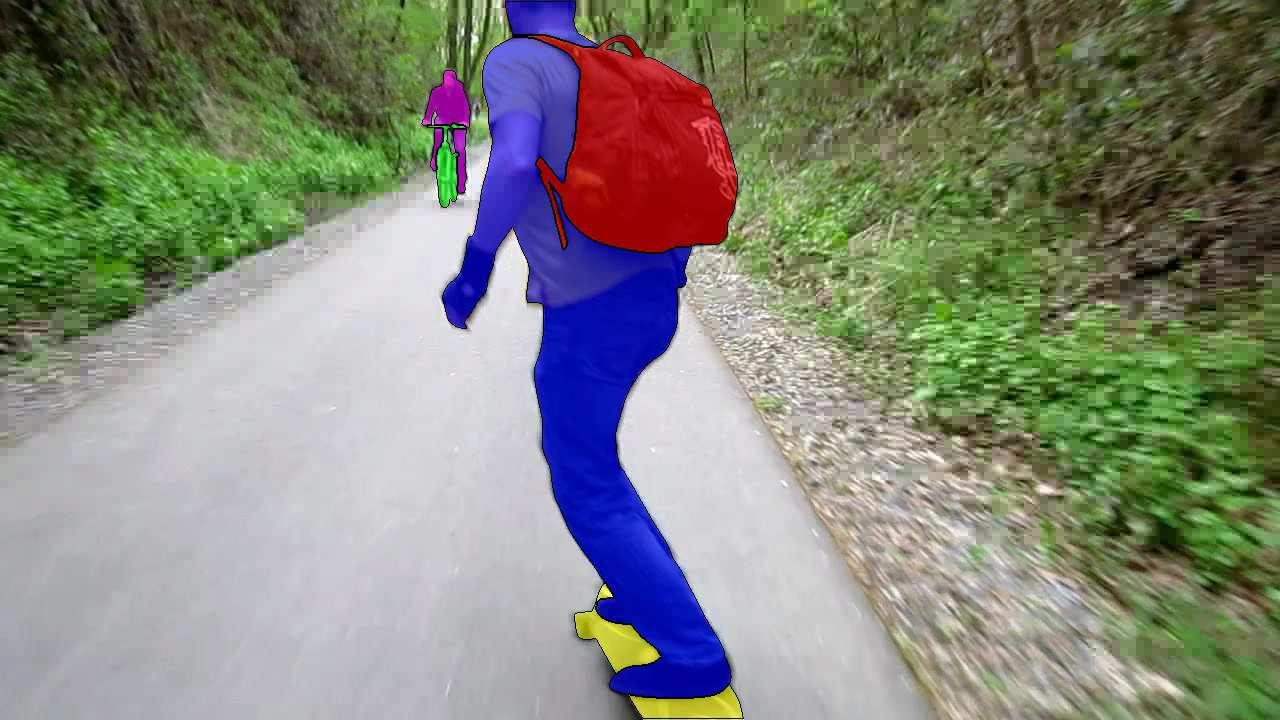
\includegraphics[width=1.\linewidth]{figures/davis_dataset/image_1.jpg}
\end{subfigure}%
\begin{subfigure}{.25\textwidth}
  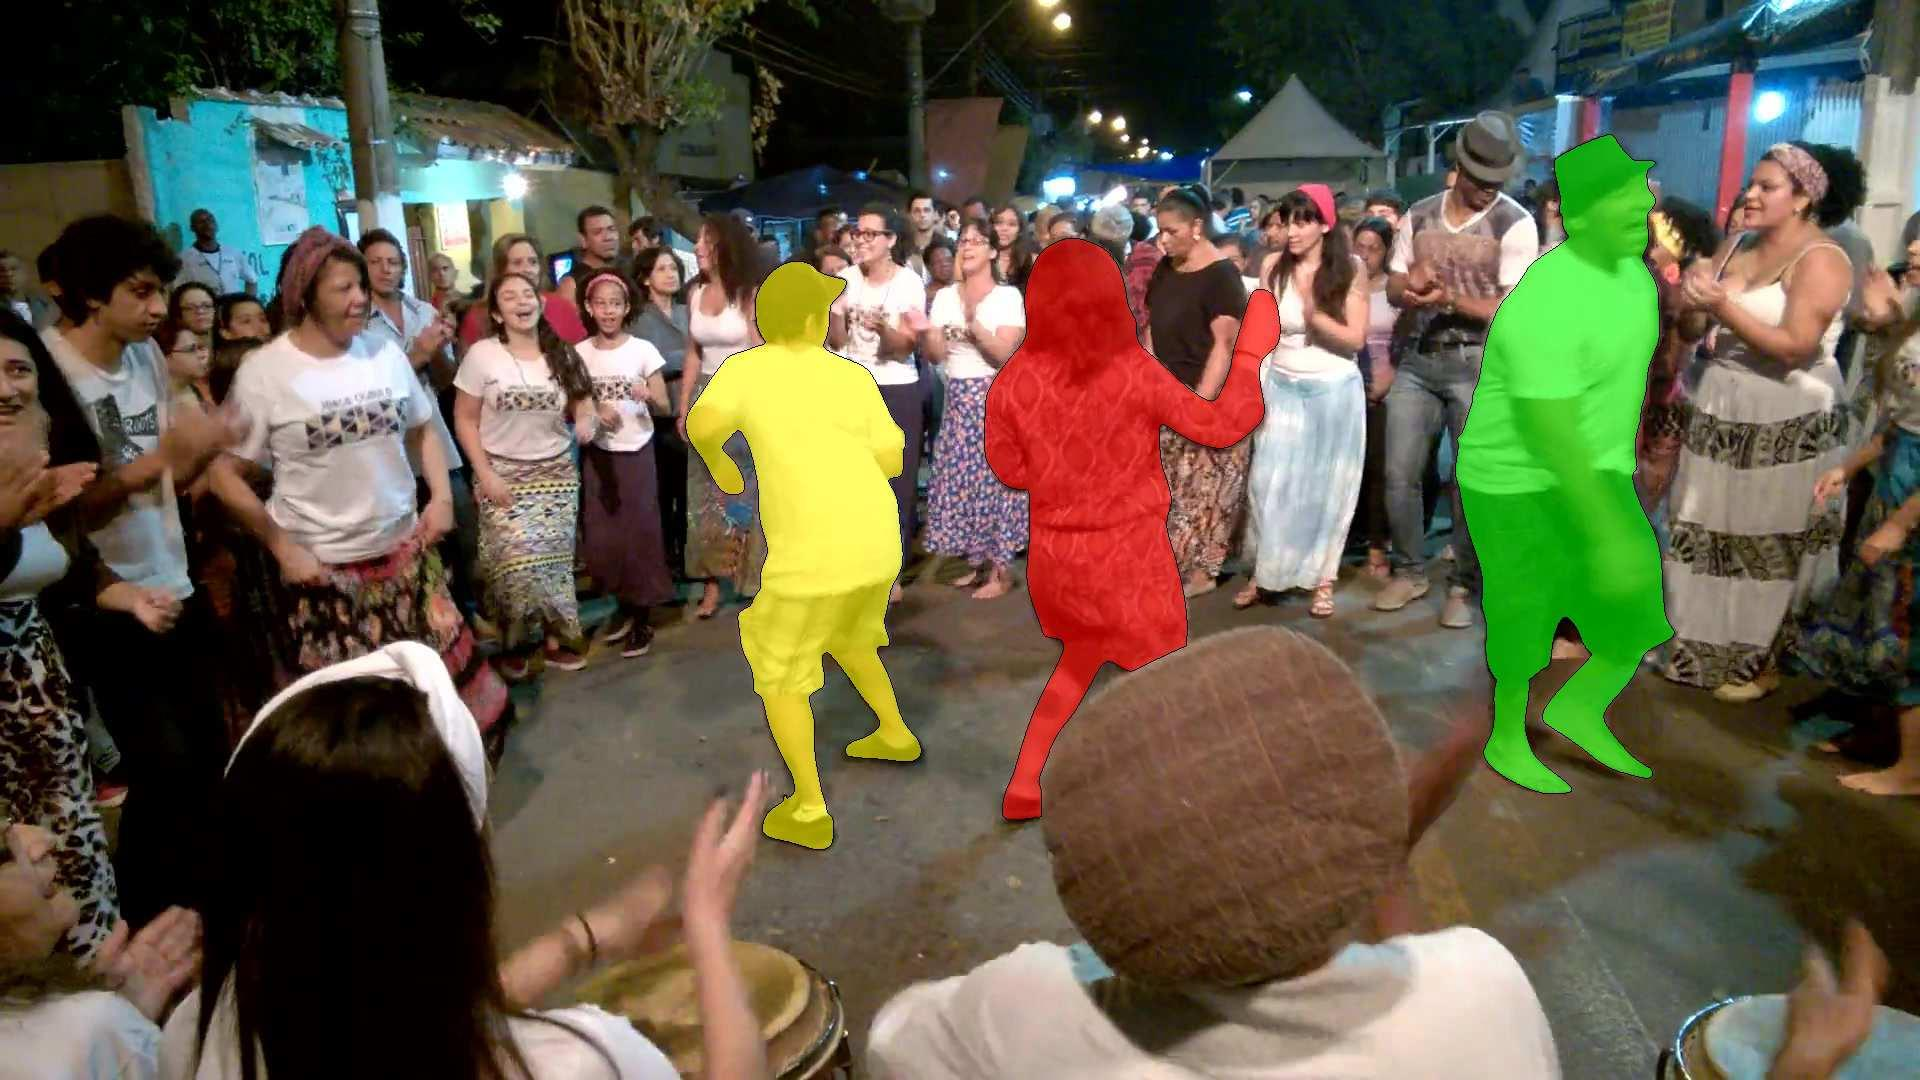
\includegraphics[width=1.\linewidth]{figures/davis_dataset/image_2.jpg}
\end{subfigure}%
\begin{subfigure}{.25\textwidth}
  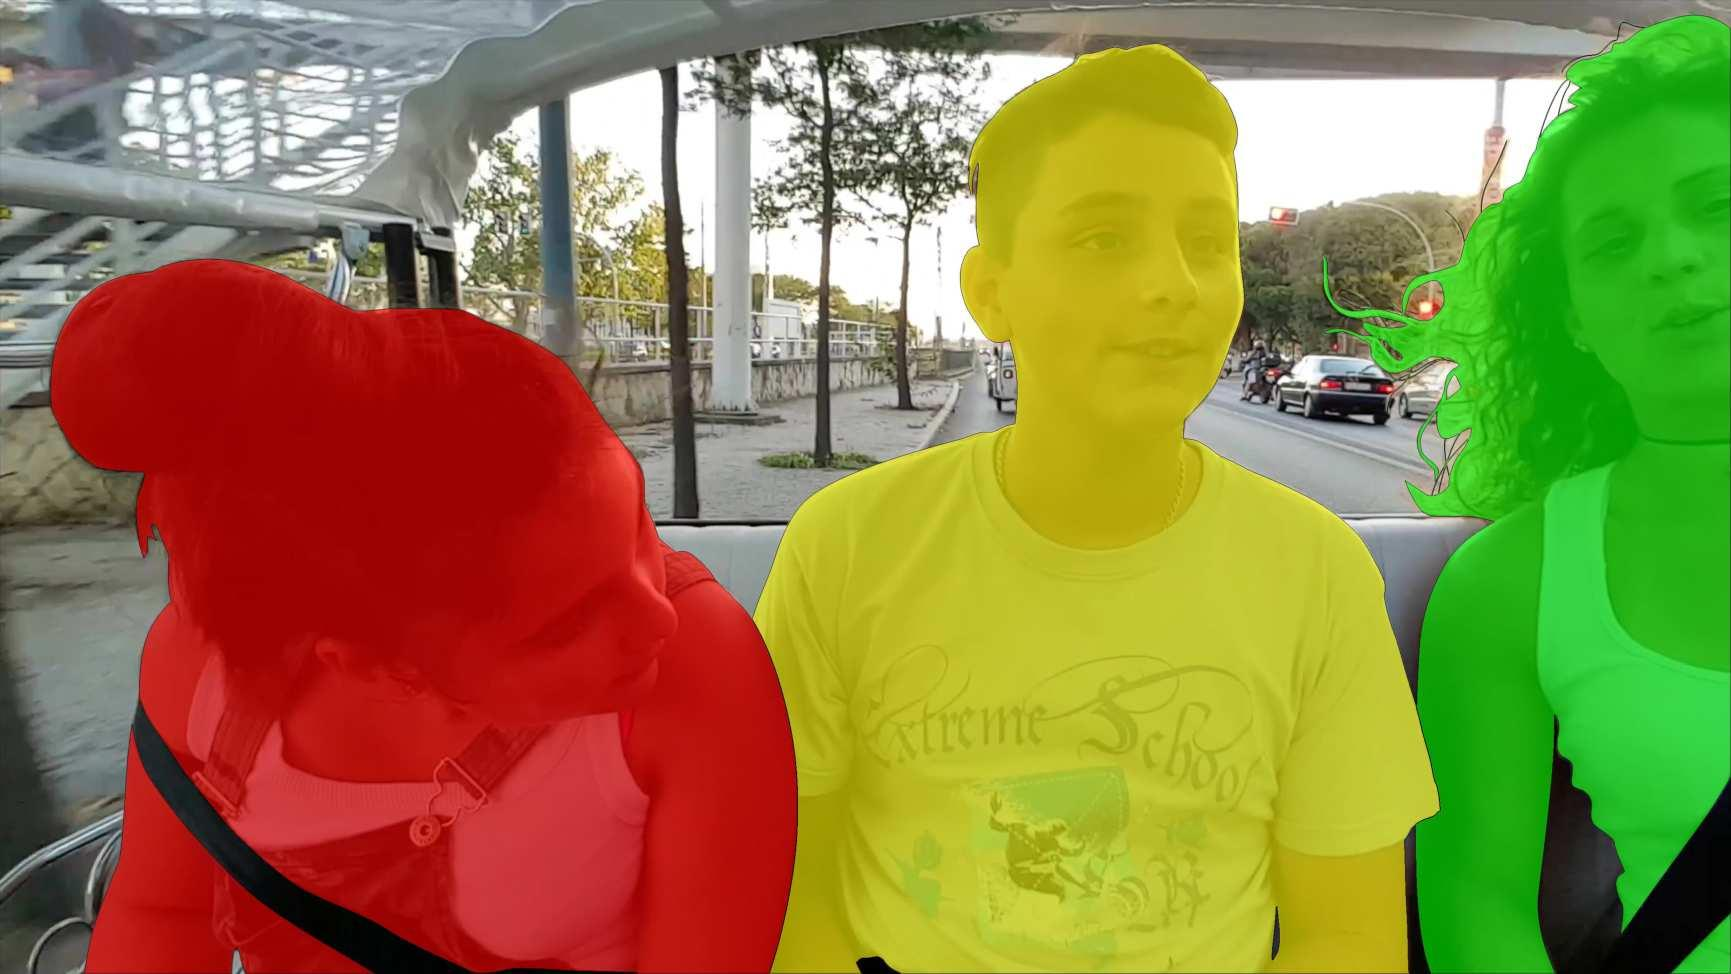
\includegraphics[width=1.\linewidth]{figures/davis_dataset/image_3.jpg}
\end{subfigure}%
\begin{subfigure}{.25\textwidth}
  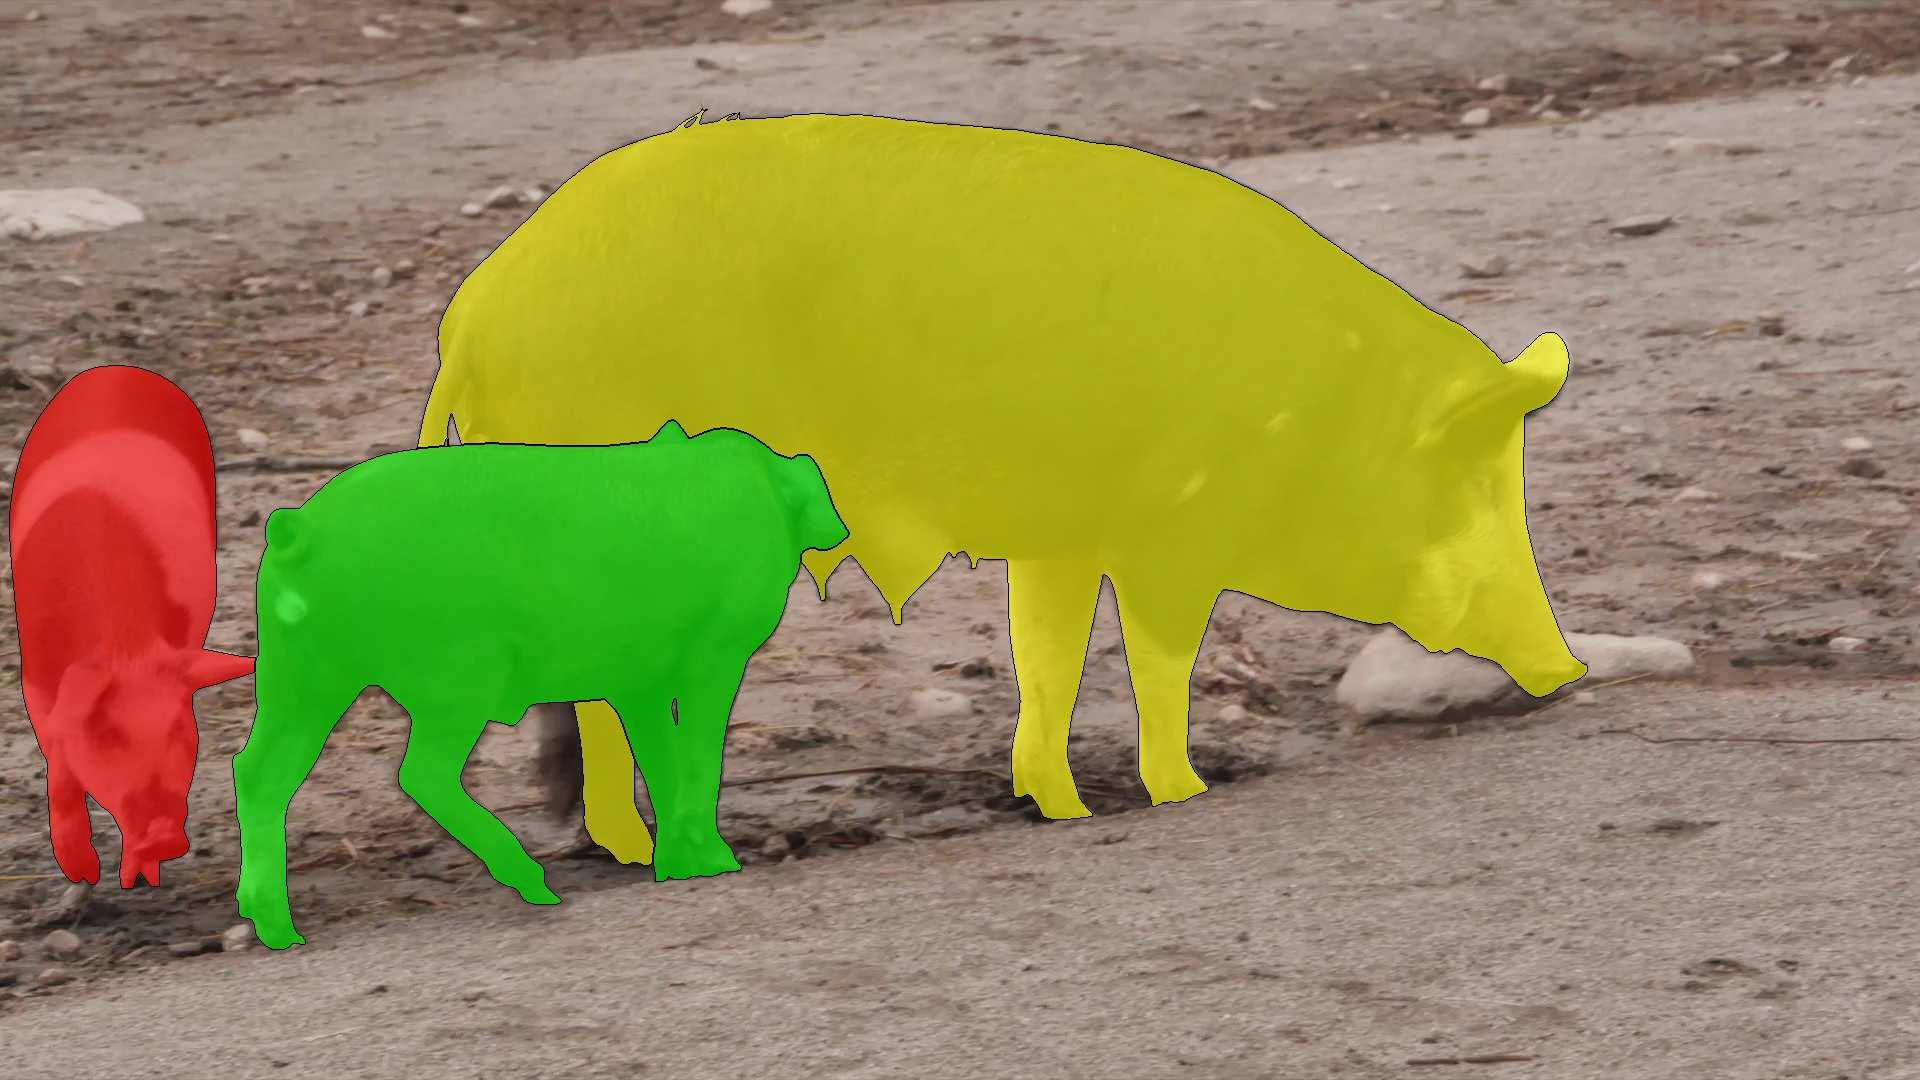
\includegraphics[width=1.\linewidth]{figures/davis_dataset/image_4.jpg}
\end{subfigure}
\caption{Example of annotations on DAVIS 2017 Dataset.}
\label{fig:davis}
\end{figure}


The DAVIS dataset owners also organize a challenge to evaluate the performance of different segmentation method.
This challenge have two branches which are the following:

\paragraph{Semi-supervised}

Consists on generate a prediction given only the ground truth mask of the first frame.
This gives information to the about which is the object intended to be segmented.

\paragraph{Unsupervised}

As the name specifies, no information is given about the object that must be segmented.
To solve this, the segmentation methods rely on the frames to infer the foreground and background.

\subsection{PASCAL Dataset}

PASCAL Dataset~\cite{Everingham10} is a dataset used to benchmark vision object category recognition, detections and segmentation.
Consist on images containing 20 visual object classes and provides multiple annotation for different computer vision tasks: detection and segmentation.
The segmentation annotations consist on masks over instances belonging to the 20 classes, which lead with images with multiple instance annotations.

During this thesis, the segmentation annotations from PASCAL VOC 2012 have been used. The information about the number of instances per split can be found on \tabref{pascal} and some samples of the dataset at \figref{pascal}.

\begin{table}[h]
\centering
\begin{tabular}{l|lll}
PASCAL VOC 2012                    & train & val  & \textbf{Total} \\
\hline
Number of images                & 1464    & 1449   & \textbf{2913}    \\
Number of instances           & 3507 & 3427 & \textbf{6934} \\
Mean number of instances per image & 2.40  & 2.37 & \textbf{2.38}  \\
\end{tabular}
\caption{Size of the PASCAL VOC 2012 data splits: number of images and annotated objects.}
\label{tab:pascal}
\end{table}


\begin{figure}[h]
\centering
% Images
\begin{subfigure}{.25\textwidth}
  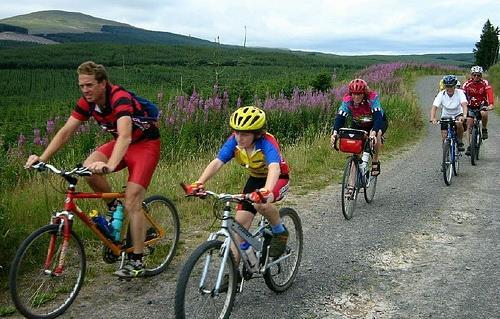
\includegraphics[width=1.\linewidth,height=0.618\linewidth]{figures/pascal_dataset/image-1.jpg}
\end{subfigure}%
\begin{subfigure}{.25\textwidth}
  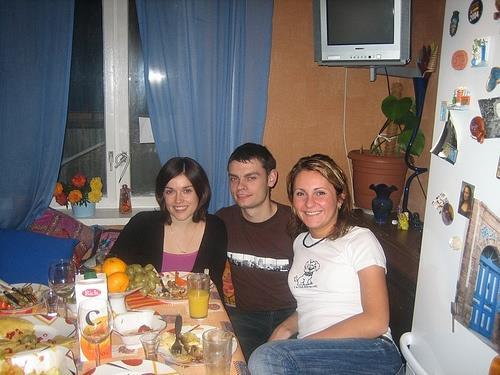
\includegraphics[width=1.\linewidth,height=0.618\linewidth]{figures/pascal_dataset/image-2.jpg}
\end{subfigure}%
\begin{subfigure}{.25\textwidth}
  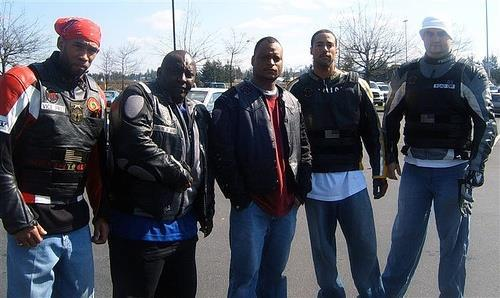
\includegraphics[width=1.\linewidth,height=0.618\linewidth]{figures/pascal_dataset/image-3.jpg}
\end{subfigure}%
\begin{subfigure}{.25\textwidth}
  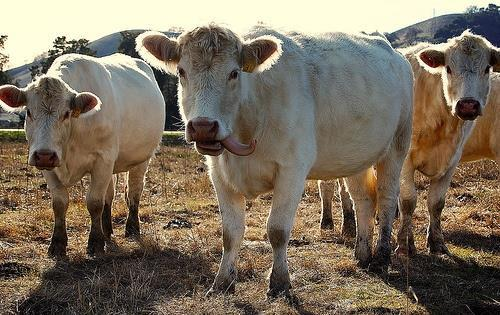
\includegraphics[width=1.\linewidth,height=0.618\linewidth]{figures/pascal_dataset/image-4.jpg}
\end{subfigure}
% Annotations
\begin{subfigure}{.25\textwidth}
  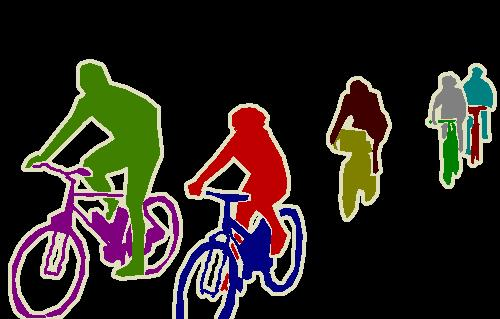
\includegraphics[width=1.\linewidth,height=0.618\linewidth]{figures/pascal_dataset/annotation-1.jpg}
\end{subfigure}%
\begin{subfigure}{.25\textwidth}
  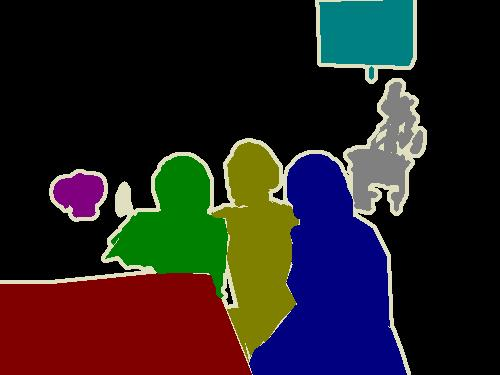
\includegraphics[width=1.\linewidth,height=0.618\linewidth]{figures/pascal_dataset/annotation-2.jpg}
\end{subfigure}%
\begin{subfigure}{.25\textwidth}
  
\includegraphics[width=1.\linewidth,height=0.618\linewidth]{figures/pascal_dataset/annotation-3.jpg}
\end{subfigure}%
\begin{subfigure}{.25\textwidth}
  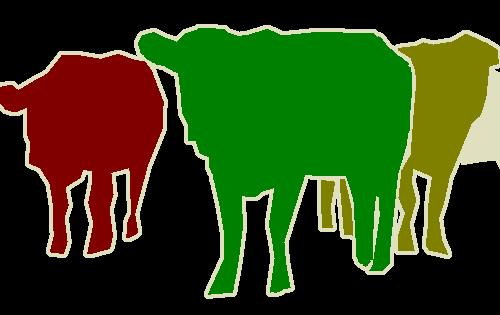
\includegraphics[width=1.\linewidth,height=0.618\linewidth]{figures/pascal_dataset/annotation-4.jpg}
\end{subfigure}
\caption{Example of images (top) and annotations (bottom) on PASCAL VOC 2012 Dataset.}
\label{fig:pascal}
\end{figure}


%%%%%%%%%%%%%%%%%%%%%%%%%%%%%%%%%

\section{Experiments}

\subsection{Tracking}

List all the experiments and its results regarding the tracking points on DAVIS\@.
Put mostly the results in the dashboard here.

Show the results of tracking points using triplet sampling. Improving the coverage.

Then the results pivoting to instance segmentation. Put here the results of the notebook.


\begin{figure}[h]
	\centering
	%!TEX root = ../thesis.tex

\begin{tikzpicture}
  \begin{axis}[
      set layers,
      width=\textwidth,
      height=.5\textwidth,
      width=\linewidth, % Scale the plot to \linewidth
      grid=both,
      grid style=dotted,
      minor ytick={0,0.05,...,1.1},
      ytick={0,0.1,...,1.1},
      yticklabels={0,.1,.2,.3,.4,.5,.6,.7,.8,.9,1},
      ymin=0, ymax=1,
      xmin=0, xmax=50,
      xlabel=Distance (pixels), % Set the labels
      ylabel=Detection Rate,
      legend columns=1,
      %transpose legend,
      cycle list name=exotic,
      legend pos= south east,
      legend style={/tikz/every even column/.append style={column sep=3mm}},
      % legend style={at={(0.5,-0.2)},anchor=north},
      % x tick label style={rotate=90,anchor=east}
    ]
    \addplot+[smooth, cyan, mark=none, line width=1]
    table [x=Threshold, y=Baseline, col sep=comma] {data/precission_threshold_curves.csv};
    \addlegendentry{Baseline}

    \addplot+[smooth, red, mark=none, line width=1]
    table [x=Threshold, y=MDNet, col sep=comma] {data/precission_threshold_curves.csv};
    \addlegendentry{MDNet}

    % \addplot+[smooth, green, mark=none, line width=1]
    % table [x=Threshold, y=Hourglass w/o Parent Network 1HG x2 sigma 5, col sep=comma] {data/precission_threshold_curves.csv};
    % \addlegendentry{Hourglass}

    % \addplot+[smooth,  mark=none, line width=1]
    % table [x=Threshold, y=ResNet101 sigma20, col sep=comma] {data/precission_threshold_curves.csv};
    % \addlegendentry{ResNet101}

    \addplot+[smooth,  mark=none, line width=1]
    table [x=Threshold, y=ResNet50 sigma40, col sep=comma] {data/precission_threshold_curves.csv};
    \addlegendentry{ResNet50}

    \addplot+[smooth,  mark=none, line width=1]
    table [x=Threshold, y=ResNet50 Multiscale sigma964824, col sep=comma] {data/precission_threshold_curves.csv};
    \addlegendentry{ResNet50 Multiscale}

  \end{axis}
\end{tikzpicture}

  \label{fig:tracking_point_regression}
	\caption{Precission performance for point regression.}
\end{figure}


Tracking the features vector of the ResNet101 pretrained with VOC\@.
The best tracking was performed using cosine distance and averaging the representation of $3 \times 3$ patches.
Backbone architecture ResNet101.

\begin{figure}[h]
  \centering
  %!TEX root = ../thesis.tex

\begin{tikzpicture}
  \begin{axis}[
      set layers,
      width=\textwidth,
      height=.5\textwidth,
      width=\linewidth, % Scale the plot to \linewidth
      grid=both,
      grid style=dotted,
      minor ytick={0,0.05,...,1.1},
      ytick={0,0.1,...,1.1},
      yticklabels={0,.1,.2,.3,.4,.5,.6,.7,.8,.9,1},
      ymin=0, ymax=1,
      xmin=0, xmax=50,
      xlabel=Distance (pixels), % Set the labels
      ylabel=Detection Rate,
      legend columns=1,
      %transpose legend,
      cycle list name=exotic,
      legend pos= north west,
      legend style={/tikz/every even column/.append style={column sep=3mm}},
      % legend style={at={(0.5,-0.2)},anchor=north},
      % x tick label style={rotate=90,anchor=east}
    ]

    % \addplot+[smooth,  mark=none, line width=1]
    %   table [x=Threshold, y=Features Metric Learning Quadplet Loss (480p) Basic metriccosine patchsize3, col sep=comma] {data/precission_threshold_curves.csv};
    % \addlegendentry{Double Triplet Loss D=2048}

    \addplot+[smooth,  mark=none, line width=1]
      table [x=Threshold, y=Features Metric Learning Triplet Loss (480p) D128 Basic metriccosine patchsize3, col sep=comma] {data/precission_threshold_curves.csv};
    \addlegendentry{Triplet Loss D=128}

    \addplot+[smooth,  mark=none, line width=1]
      table [x=Threshold, y=Features Metric Learning (480p) Basic metriccosine patchsize3, col sep=comma] {data/precission_threshold_curves.csv};
    \addlegendentry{Triplet Loss D=2048}

    \addplot+[smooth,  mark=none, line width=1]
    table [x=Threshold, y=Features ResNet Basic metriccosine patchsize3, col sep=comma] {data/precission_threshold_curves.csv};
    \addlegendentry{Pre-Trained VOC D=2048}

    \addplot+[smooth,  mark=none, line width=1]
    table [x=Threshold, y=Baseline, col sep=comma] {data/precission_threshold_curves.csv};
    \addlegendentry{Baseline}

  \end{axis}
\end{tikzpicture}

  \label{fig:tracking_metric_learning}
  \caption{Precission performance for pixel representation tracking.}
\end{figure}

%!TEX root = ../thesis.tex

\chapter{Conclusion and Future Work}
\label{cha:conclusionsfuturework}

In this Master Thesis, we have tackled the task if weakly supervised video object segmentation, i.e., 
the segmentation of multiple objects of interest in a video sequence given a point per object in the first frame.
We have presented several methods and combined two of them to obtain the final solution.
First, we have presented two ways to track a point on a video sequence.
The first approach consisted in training a model per each video sequence, 
using the first frame and the point to track represented as a heatmap.
This method presented good precision and coverage results. 
However, its major weaknesses are its speed and generalization as a model has to be trained for every new sequence.

The second approach presented to track points consisted in training an embedding model which outputs an embedding representation for every pixel.
The training was performed using metric learning, more specifically, the Triplet Loss was used and the distances to the initial point was computed.
Despite of the fact that precision was low, the coverage result was as good as in the previous method.
This model was completely sequence agnostic and it could perform fast inference without any additional training.

After being able to track points, the following method consisted in obtaining the mask of an object given a point belonging to it.
We decided to use the embedding model used to track the points as it provided a good embedding quality.
We tested different margins of the Triplet Loss in order to obtain the best segmentation performance possible.
This model presented good results in many situation where multiple objects, even from the same class, 
could be distinguished as different instances.
On the other hand, 
this model presented low performance when small objects had to be segmented and also the quality of the pixels of the embeddings close to object contours was not very good.

We combined the two metric learning approaches to perform video object segmentation by tracking a point. The final performance falls behind the current state of the art semi-supervised methods, but we have to take into account that we are only using a point and not the full mask in the first frame to perform the segmentation in the rest of the video sequence.
The main weakness of our method is in tracking the points. The performance of our model drops when the object to track in the first frame is very small, also occlusions pose a difficult challenge.
A possible solution to mitigate these drawbacks is to train and infer the embeddings using multiple scales of an image as has been done previously in the literature.
This could lead to a model that outputs an embedding with more contextual information on each pixel embedding, which can lead to an increase in performance on tracking and segmenting.

To conclude, we believe that the presented method could lead to promising results in the segmentation field when using embedding representation of pixels, but further exploration is required. 



%% ----------------------------------------------------------------------------
% If Appendix is needed
%% ----------------------------------------------------------------------------
\appendix
%!TEX root = ../thesis.tex

%% ----------------------------------------------------------------------------
% BIWI SA/MA thesis template
%
% Created 09/29/2006 by Andreas Ess
% Extended 13/02/2009 by Jan Lesniak - jlesniak@vision.ee.ethz.ch
%% ----------------------------------------------------------------------------
\chapter{The First Appendix}

In the appendix, list the following material:

\begin{itemize}
 \item Data (evaluation tables, graphs etc.)
 \item Program code
 \item Further material
\end{itemize}


%% ----------------------------------------------------------------------------
% Bibliography is stored in references.bib file, and can often be found
% online on webpages like dblp.uni-trier.de
%
% To include it in your thesis, run
%  pdflatex main
%  bibtex main
%  pdflatex main
%  pdflatex main
%
% This ensures all references are done correctly.
%% ----------------------------------------------------------------------------

\bibliographystyle{amsalpha}
\bibliography{references}

\end{document}
